\chapter{Polynomial-Time Reductions and NP}

\tikzset{rv/.style={circle, draw, thick, minimum size=6mm, inner sep=0pt, font=\small},
  rw/.style={font=\scriptsize, fill=white, text=black, inner sep=1pt}}

So far we found efficient algorithms. For many natural problems (e.g.\ 0/1 knapsack without a pseudo-polynomial bound, travelling salesman,
3-colouring) nobody knows a polynomial-time algorithm. The theory of NP-completeness lets us show that such problems are all
equally hard, so that a fast algorithm for one would give fast algorithms for all.

\section{Decision problems and P}
\begin{definition}
A \emph{decision problem} is a problem whose answer is yes or no. Formally it is a set $L$ of (encoded) instances, the yes-instances;
an algorithm \emph{solves} $L$ if it outputs yes exactly on inputs in $L$.
\end{definition}
Optimization problems have decision versions obtained by adding a threshold:
\begin{itemize}
  \item \textsc{Independent-Set}: given $G$ and $k$, does $G$ have an independent set of size $\ge k$?
  \item \textsc{TSP}: given complete weighted graph and $B$, is there a tour of total weight $\le B$?
\end{itemize}
The decision version is no harder than the optimization version, and usually not much easier: e.g.\ binary search on $k$ finds the optimal value with
$\bigO(\log n)$ calls, and self-reducibility recovers an optimal solution.

\begin{definition}
$\mathbf{P}$ is the class of decision problems solvable in time $\bigO(n^c)$ for some constant $c$, where $n$ is the input size in bits.
\end{definition}
Why polynomial? The class is closed under composition: an algorithm that runs in polynomial time and calls a polynomial-time subroutine polynomially many times is still polynomial. It is also
robust across reasonable machine models, and in practice polynomial algorithms usually have small exponents.

\begin{important}[Input size, again]
\textsc{Knapsack} with $\Theta(nW)$ is not known to be in P: $W$ takes $\log W$ bits. Similarly, trial division to test primality of $N$ takes
$\sqrt N=2^{(\log N)/2}$ steps, which is exponential. (Primality \emph{is} in P, by AKS 2002.)
\end{important}

\section{Polynomial-time reductions}
\begin{definition}[Many-one / Karp reduction]
$A\le_P B$ if there is a polynomial-time computable function $f$ mapping instances of $A$ to instances of $B$ such that
\[
x\in A\iff f(x)\in B.
\]
\end{definition}
\begin{lemma}
\begin{enumerate}
  \item If $A\le_PB$ and $B\in\mathbf P$, then $A\in\mathbf P$.
  \item (Contrapositive) If $A\le_PB$ and $A\notin\mathbf P$, then $B\notin\mathbf P$.
  \item $\le_P$ is transitive.
\end{enumerate}
\end{lemma}
\begin{proof}
(1) On input $x$, compute $f(x)$ in time $p(|x|)$; then $|f(x)|\le p(|x|)$, and run $B$'s algorithm in time $q(p(|x|))$, a polynomial.
(3) Compose the two functions; a polynomial of a polynomial is a polynomial.
\end{proof}

\begin{figure}[H]
\centering
\begin{tikzpicture}[>=Stealth, thick, font=\small,
  blk/.style={draw, rounded corners, fill=blue!6, minimum height=1cm, align=center}]
  \node[blk] (f) at (0,0) {compute $f$\\{\scriptsize poly time}};
  \node[blk] (b) at (4,0) {algorithm\\for $B$};
  \draw[->] (-2.4,0) node[left]{$x$} -- (f);
  \draw[->] (f) -- node[above]{$f(x)$} (b);
  \draw[->] (b.east) -- ++(0.8,0.4) node[right]{yes};
  \draw[->] (b.east) -- ++(0.8,-0.4) node[right]{no};
  \draw[densely dashed, rounded corners] (-1.6,-1) rectangle (5.6,1.1);
  \node[font=\scriptsize, anchor=south east] at (5.6,1.1) {algorithm for $A$};
\end{tikzpicture}
\caption{A reduction $A\le_P B$ turns any algorithm for $B$ into one for
$A$ with the same answer, since $x\in A\iff f(x)\in B$.}
\end{figure}

\begin{important}[Direction]
$A\le_PB$ means ``$A$ is no harder than $B$''. To show a new problem $X$ is hard, reduce a \emph{known hard} problem \emph{to} $X$.
A reduction must handle \emph{every} instance of $A$, and you must prove \emph{both} directions of the iff.
\end{important}

(Sometimes Cook/Turing reductions are used: solve $A$ in polynomial time given an oracle for $B$. For NP-completeness, CS 341 uses Karp reductions.)

\subsection{First examples}
\begin{definition}
In a graph $G=(V,E)$: $S\subseteq V$ is \emph{independent} if no edge has both ends in $S$; $C\subseteq V$ is a \emph{vertex cover} if every edge has at least
one end in $C$; $K\subseteq V$ is a \emph{clique} if every pair in $K$ is adjacent.
\end{definition}

\begin{lemma}
$S$ is independent in $G$ iff $V\setminus S$ is a vertex cover iff $S$ is a clique in the complement $\overline G$.
\end{lemma}
\begin{proof}
$S$ independent $\iff$ no edge inside $S$ $\iff$ every edge has an end outside $S$ $\iff$ $V\setminus S$ covers every edge.
And no edge of $G$ inside $S$ $\iff$ every pair in $S$ is an edge of $\overline G$.
\end{proof}

\begin{figure}[H]
\centering
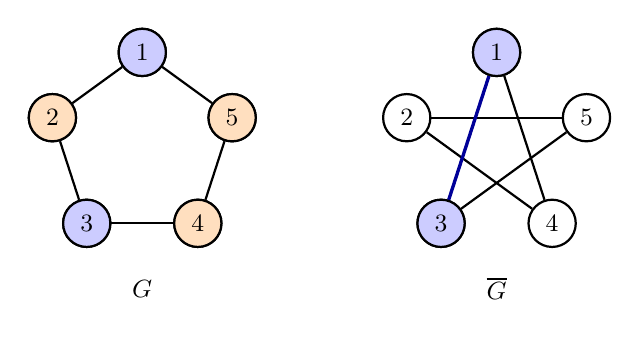
\begin{tikzpicture}[font=\small]
  \foreach \i in {1,...,5} \node[rv] (a\i) at ({90+72*(\i-1)}:1.2) {\i};
  \foreach \i/\j in {1/2, 2/3, 3/4, 4/5, 5/1} \draw[thick] (a\i) -- (a\j);
  \foreach \i in {1,3} \node[rv, fill=blue!20] at (a\i) {\i};
  \foreach \i in {2,4,5} \node[rv, fill=orange!25] at (a\i) {\i};
  \node at (0,-1.8) {$G$};
  \begin{scope}[xshift=4.5cm]
    \foreach \i in {1,...,5} \node[rv] (b\i) at ({90+72*(\i-1)}:1.2) {\i};
    \foreach \i/\j in {1/3, 3/5, 5/2, 2/4, 4/1} \draw[thick] (b\i) -- (b\j);
    \draw[very thick, blue!60!black] (b1) -- (b3);
    \foreach \i in {1,3} \node[rv, fill=blue!20] at (b\i) {\i};
    \node at (0,-1.8) {$\overline G$};
  \end{scope}
\end{tikzpicture}
\caption{In the 5-cycle $G$, $S=\{1,3\}$ (blue) is independent, its
complement $\{2,4,5\}$ (orange) is a vertex cover, and in $\overline G$
the set $S$ is a clique.}
\end{figure}

\begin{theorem}
$\textsc{Independent-Set}\equiv_P\textsc{Vertex-Cover}\equiv_P\textsc{Clique}$.
\end{theorem}
\begin{proof}
$(G,k)\in\textsc{IS}\iff(G,n-k)\in\textsc{VC}$, and $(G,k)\in\textsc{IS}\iff(\overline G,k)\in\textsc{Clique}$. These maps are computable in polynomial time
($\overline G$ takes $\bigO(n^2)$). The reverse reductions are symmetric.
\end{proof}

\begin{example}[Reduction to a more general problem]
\textsc{Vertex-Cover}$\le_P$\textsc{Set-Cover}: given $(G,k)$, let the universe be $E$ and for each vertex $v$ create the set of edges incident to $v$.
A set cover of size $k$ is exactly a vertex cover of size $k$.
\end{example}

\begin{example}[Hamiltonian cycle to TSP]
\textsc{Ham-Cycle}: does $G$ have a cycle through every vertex exactly once? Given $G$, build the complete graph on $V$ with $w(u,v)=1$ if $uv\in E$ and $2$ otherwise, and set $B=n$.
A tour of weight $\le n$ uses only weight-1 edges, i.e.\ is a Hamiltonian cycle in $G$; conversely a Hamiltonian cycle is a tour of weight $n$.
\end{example}

\begin{center}
\begin{tikzpicture}[x=1.8cm, y=1.6cm, font=\small]
  \node[rv] (a) at (0,1) {$a$}; \node[rv] (b) at (1,1) {$b$}; \node[rv] (c) at (1,0) {$c$}; \node[rv] (d) at (0,0) {$d$};
  \foreach \u/\v in {a/b, b/c, c/d, d/a, a/c} \draw[thick] (\u) -- (\v);
  \node at (0.5,-0.6) {$G$};
  \draw[->, thick, >=Stealth] (1.4,0.5) -- (2.0,0.5);
  \begin{scope}[xshift=4.3cm]
    \node[rv] (a2) at (0,1) {$a$}; \node[rv] (b2) at (1,1) {$b$}; \node[rv] (c2) at (1,0) {$c$}; \node[rv] (d2) at (0,0) {$d$};
    \foreach \u/\v in {a2/b2, b2/c2, c2/d2, d2/a2} \draw[very thick, blue!60!black] (\u) -- node[rw]{1} (\v);
    \draw[thick] (a2) -- node[rw, pos=0.3]{1} (c2);
    \draw[thick, densely dashed] (b2) -- node[rw, pos=0.3]{2} (d2);
    \node at (0.5,-0.6) {TSP instance, $B=4$};
  \end{scope}
\end{tikzpicture}
\end{center}
The Hamiltonian cycle $a,b,c,d$ of $G$ becomes a tour of weight exactly
$4=n$; the non-edge $bd$ gets weight 2.

\section{NP}
\begin{definition}
A decision problem $L$ is in $\mathbf{NP}$ if there is a polynomial-time algorithm $V$ (the \emph{verifier}) and a polynomial $p$ such that
\[
x\in L\iff\exists\,y\text{ with }|y|\le p(|x|)\text{ such that }V(x,y)\text{ accepts}.
\]
Such a $y$ is a \emph{certificate} (witness) for $x$.
\end{definition}
In words: yes-instances have short proofs that can be checked quickly. No-instances need not have short proofs.
(NP stands for \emph{nondeterministic polynomial time}: a nondeterministic machine can guess $y$ and run $V$.)

\begin{example}
\begin{itemize}
  \item \textsc{Independent-Set}$\in$NP: certificate is the set $S$; check $|S|\ge k$ and no edge inside $S$ in $\bigO(n+m)$.
  \item \textsc{Ham-Cycle}$\in$NP: certificate is an ordering of $V$; check it is a permutation and consecutive vertices (cyclically) are adjacent.
  \item \textsc{SAT}$\in$NP: certificate is a truth assignment; evaluate the formula.
  \item \textsc{Composite} ($N$ is not prime) $\in$NP: certificate is a nontrivial factor.
\end{itemize}
\end{example}

\begin{theorem}
$\mathbf P\subseteq\mathbf{NP}$.
\end{theorem}
\begin{proof}
If $L\in\mathbf P$ via algorithm $A$, take the verifier $V(x,y)=A(x)$ that ignores the certificate (use the empty certificate).
\end{proof}
Also $\mathbf{NP}\subseteq\mathbf{EXP}$: try all $2^{p(n)}$ certificates.

\paragraph{co-NP.} $\mathbf{coNP}=\{\overline L: L\in\mathbf{NP}\}$: problems whose \emph{no}-instances have short certificates, e.g.\ \textsc{Tautology}, or
``$G$ has no Hamiltonian cycle''. It is unknown whether $\mathbf{NP}=\mathbf{coNP}$.

\begin{important}[The big question]
Is $\mathbf P=\mathbf{NP}$? I.e.\ is finding a solution as easy as checking one? It is widely believed that $\mathbf P\ne\mathbf{NP}$, but this is open
(a Clay Millennium Prize problem).
\end{important}

\section{NP-hard and NP-complete}
\begin{definition}
$B$ is \textbf{NP-hard} if $A\le_PB$ for every $A\in\mathbf{NP}$. $B$ is \textbf{NP-complete} if moreover $B\in\mathbf{NP}$.
\end{definition}
\begin{lemma}
If some NP-complete problem is in P, then $\mathbf P=\mathbf{NP}$. If $A$ is NP-complete, $B\in\mathbf{NP}$, and $A\le_PB$, then $B$ is NP-complete.
\end{lemma}
\begin{proof}
The first follows from the reduction lemma. For the second, any $L\in\mathbf{NP}$ has $L\le_PA\le_PB$, and $\le_P$ is transitive.
\end{proof}

\begin{center}
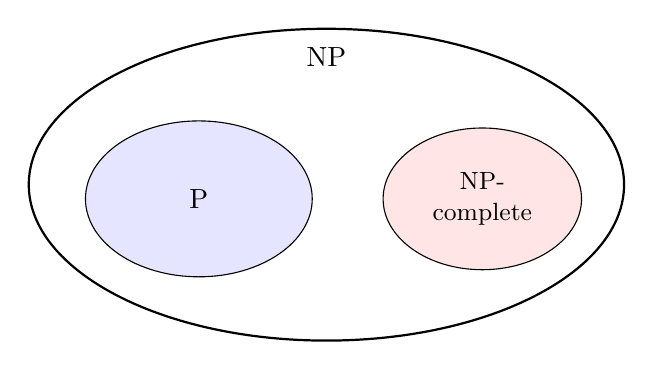
\begin{tikzpicture}[scale=0.9]
\draw[thick] (0,0) ellipse (4.2 and 2.2);
\node at (0,1.8) {NP};
\draw[fill=blue!10] (-1.8,-0.2) ellipse (1.6 and 1.1);
\node at (-1.8,-0.2) {P};
\draw[fill=red!10] (2.2,-0.2) ellipse (1.4 and 1.0);
\node[align=center,font=\small] at (2.2,-0.2) {NP-\\complete};
\end{tikzpicture}

{\small The picture if $\mathbf P\ne\mathbf{NP}$ (Ladner: then there are also NP problems that are neither in P nor NP-complete).}
\end{center}

\begin{important}[Recipe: proving $X$ is NP-complete]
\begin{enumerate}
  \item Show $X\in\mathbf{NP}$: describe the certificate and the polynomial-time verifier.
  \item Choose a known NP-complete problem $Y$.
  \item Give a polynomial-time construction $f$ mapping instances of $Y$ to instances of $X$.
  \item Prove: $y\in Y\Rightarrow f(y)\in X$ (turn a solution of $y$ into a solution of $f(y)$).
  \item Prove: $f(y)\in X\Rightarrow y\in Y$ (turn a solution of $f(y)$ back into a solution of $y$). This is usually the harder direction.
  \item Argue $f$ runs in polynomial time (size of the construction).
\end{enumerate}
\end{important}

\section*{Summary}
\begin{itemize}
  \item Decision problems; P = polynomial time in the number of input bits.
  \item $A\le_PB$: polynomial-time map preserving yes/no answers; reduce \emph{from} the known hard problem.
  \item NP = problems with polynomial-size, polynomial-time verifiable certificates for yes-instances; $\mathbf P\subseteq\mathbf{NP}$.
  \item NP-complete = in NP and every NP problem reduces to it. IS, VC, Clique are polynomially equivalent.
\end{itemize}
